\section{Results and Discussion}\label{sec:results}
This section first reports how the policies performed in simulation and on the real robot.
It then compares the sim-to-real gap of the two branches, which is the main question of this
study, and finally looks at why the real robot failed on most routes.

\subsection{Simulation Results}
Table~\ref{tab:sim} shows the final simulated performance of all six policies, each evaluated over
five sessions of the 20 routes. The standard policies performed better in simulation, with a mean SR
of 0.58 against 0.42 for photogrammetry. The seeds also varied considerably: standard seed~2 reached
only 0.39, while seeds 0 and 1 both reached 0.67. A likely reason for the lower photogrammetry
scores is that its world is harder to navigate: the scanned obstacles have irregular shapes, and the
mesh has small cracks that leave gaps in the depth image (Fig.~\ref{fig:worlds}; appendix,
Fig.~\ref{fig:depth}), whereas the standard world contains only clean boxes. The training curves are
given in the appendix (Fig.~\ref{fig:training}). Following the rule fixed before the real trials,
standard seed~1 and photogrammetry seed~0 were deployed on the robot.

\begin{table}[t]
\caption{Final simulated performance (mean $\pm$ standard deviation over five sessions of 20
routes). $^\ast$ marks the policy deployed on the real robot.}
\label{tab:sim}
\centering
\footnotesize
\begin{tabular}{@{}llccc@{}}
\toprule
Branch & Seed & SR & SPL & CR (per m) \\
\midrule
\multirow{4}{*}{Standard}
 & 0 & 0.67$\pm$0.06 & 0.54$\pm$0.05 & 0.09 \\
 & 1$^\ast$ & 0.67$\pm$0.08 & 0.59$\pm$0.06 & 0.17 \\
 & 2 & 0.39$\pm$0.07 & 0.37$\pm$0.06 & 0.46 \\
 & Mean & 0.58 & 0.50 & 0.24 \\
\midrule
\multirow{4}{*}{Photogrammetry}
 & 0$^\ast$ & 0.53$\pm$0.08 & 0.48$\pm$0.07 & 0.30 \\
 & 1 & 0.44$\pm$0.15 & 0.38$\pm$0.12 & 0.36 \\
 & 2 & 0.29$\pm$0.09 & 0.27$\pm$0.08 & 0.59 \\
 & Mean & 0.42 & 0.38 & 0.42 \\
\bottomrule
\end{tabular}
\end{table}

\subsection{Real-Robot Results}
Both deployed policies performed worse on the real robot than in simulation (Table~\ref{tab:real}).
By odometry-estimated success, the photogrammetry policy succeeded on 9 of 20 routes (SR
0.45) and the standard policy on 6 of 20 (SR 0.30). The
photogrammetry policy therefore did better on the real robot, but the 95\% confidence intervals
overlap, and the paired per-route comparison does not show a significant difference (SR
$p=0.18$, SPL $p=0.07$).

Collisions were rarer on the real robot than in simulation (0.032 per metre for standard and 0.055
for photogrammetry). This is mainly because NAOqi's collision protection, which was kept on for
safety, slowed or stopped the base near obstacles. Instead of colliding, the robot often stopped in
front of an obstacle until the time ran out (Section~\ref{sec:results-why}).

\begin{table}[t]
\caption{The two deployed policies in simulation and on the real robot (20 routes each). Real values are odometry-estimated. $\Delta$ is simulated
minus real; $p$ is the paired per-route Wilcoxon test.}
\label{tab:real}
\centering
\footnotesize
\setlength{\tabcolsep}{4pt}
\begin{tabular}{@{}lcc@{}}
\toprule
 & Standard (seed 1) & Photogrammetry (seed 0) \\
\midrule
Sim SR / SPL & 0.67 / 0.59 & 0.53 / 0.48 \\
Real SR & 0.30 [0.15, 0.52] & 0.45 [0.26, 0.66] \\
Real SPL & 0.16 & 0.27 \\
Real CR (per m) & 0.032 & 0.055 \\
\midrule
$\Delta$SR ($p$) & 0.37 (0.009) & 0.08 (0.392) \\
$\Delta$SPL ($p$) & 0.43 (0.001) & 0.21 (0.022) \\
\midrule
\multicolumn{3}{@{}l}{Is $\Delta_{\text{photo}} < \Delta_{\text{std}}$? SR: $p=0.03$, SPL:
$p=0.01$} \\
\bottomrule
\end{tabular}
\end{table}

\begin{figure}[t]
\centering
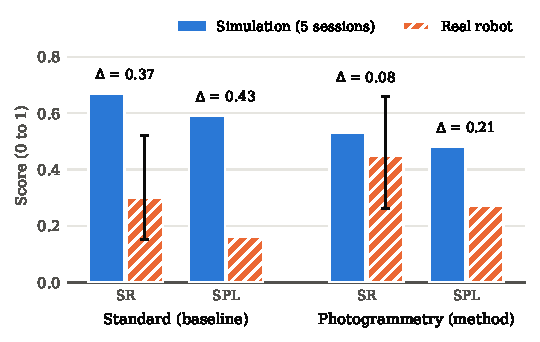
\includegraphics[width=\columnwidth]{figures/results_bars}
\caption{SR and SPL of the two deployed policies in simulation and on the real robot. Error bars on the real SR are 95\% Wilson intervals;
$\Delta$ is the sim-to-real gap.}
\label{fig:bars}
\end{figure}

\subsection{The Sim-to-Real Gap}
The photogrammetry policy lost less performance when moved to the real robot (Fig.~\ref{fig:bars}).
Its success rate fell by 8 percentage points (from 0.53 in simulation to 0.45 on the robot), while
the standard policy's fell by 37 points (from 0.67 to 0.30). Measured by SPL, which also rewards
short paths, the photogrammetry policy's drop (0.21) was about half that of the standard policy
(0.43). Comparing the two gaps route by route, the photogrammetry gap was smaller on 12 routes and
the standard gap on 3, and the difference is statistically significant ($p=0.03$ for SR, $p=0.01$
for SPL). This supports the hypothesis for the two deployed policies: the policy trained in the
photogrammetry world transferred with a smaller loss of performance. Because the test pairs routes
rather than independent training runs, it does not show that this holds across training seeds
(Section~\ref{sec:limitations}).

The smaller gap has two sources. The photogrammetry policy scored lower in simulation
(0.53 against 0.67), so its simulator gave a less optimistic prediction,
and it scored higher on the real robot (0.45 against 0.30). The standard
policy's gap was large and significant (SR $p=0.009$, SPL $p=0.001$), so its
simulator clearly over-predicted real performance. For the photogrammetry policy, only the SPL
gap was significant ($p=0.022$), while its SR gap was not ($p=0.392$): its
simulated success rate was a reasonable prediction of its real one, although it reached the goal
by less efficient paths on the real robot.

\subsection{Why the Real Robot Failed}\label{sec:results-why}
Table~\ref{tab:failures} groups every real route by how it ended, using the scored result and the
operator's notes. Two factors stand out.

\begin{table}[t]
\caption{How each real route ended (20 routes per policy)}
\label{tab:failures}
\centering
\footnotesize
\begin{tabular}{@{}lcc@{}}
\toprule
Outcome & Standard & Photogrammetry \\
\midrule
Reached the goal & 6 & 9 \\
Collided (all with the couch) & 2 & 3 \\
Stopped at the couch or bag until timeout & 5 & 5 \\
Stopped within 1\,m of the goal (near miss) & 2 & 0 \\
Barely moved ($<1$\,m) & 1 & 3 \\
Other timeout & 4 & 0 \\
\bottomrule
\end{tabular}
\end{table}

\textbf{The couch and the bag.} Many failures happened at two obstacles. The couch lies between many
of the starts and the goal, and the bag stands in the middle of the room (Fig.~\ref{fig:layout}).
Every collision was with the couch, and many more routes ended with the robot stopped in front of
the couch or the bag. In simulation, the policies reach the goal from the left of the room by
driving through the gap between the bag and the couch, passing close to the couch (appendix,
Fig.~\ref{fig:paths}). On the real robot this same gap is where most runs failed: NAOqi's collision
protection held the base back when it came close to an obstacle, while the policy kept commanding it
towards the goal. The policy had never experienced this behaviour in training, so it had not learned
to back off and try another path.

\textbf{Real-robot conditions.} The real robot also differed from the simulator in ways the
randomisation only approximated. The control loop ran at 5\,Hz over Wi-Fi with depth images at
$160\times120$, and commands took effect about 0.85\,s after they were sent. Together with the collision protection, these
conditions made the robot slower and more hesitant than in simulation, which helps explain the
many timeouts and the low SPL on the real robot.
